%!TEX root = ../thesis.tex
\section{Introduction}

Performing a software demonstration can be an effective way to communicate with the audience during a live presentation. By illustrating actions within a working system, presenters can guide the audience through an interaction flow and show results in real time. However, it is not always easy to perform an effective live demo. Problems such as software crashes, network connectivity issues, and configuration changes (e.g., screen resolution) may break a demonstration. Furthermore, talking while interacting with the system creates a high cognitive load on presenters. In addition, the stress of public speaking, especially during a high-stakes presentation, makes it difficult for presenters to deliver effective messages in a timely manner without forgetting to cover a set of core values of the system. An alternative is to present with pre-recorded screencast videos that capture the correct flow and information. Even though technical problems are less likely to occur with a video, it is challenging for presenters to talk over a video with appropriate timing because they have to mainly rely on their memories for the sequence and timing of interactions. Such a “canned” demo can often result in a less understandable or engaging presentation when a video is not tightly prepared to attract the audience's attention to anticipate the results [6].

The presenter view in PowerPoint or Keynote attempts to help presenters during slide show presentations by showing notes along with an upcoming slide. A teleprompter, commonly used for news programs or political speeches, prompts presenters with an electronic visual text of a speech or script. With this, speakers can appear to be speaking spontaneously as they look at the audience while reading the script. Inspired by these tools, we built DemoWiz (see Figure~\ref{fig:demowiz_teaser}), a system that assists presenters in giving software demonstrations with a screencast demo video during a live presentation. DemoWiz augments a screencast video with visualizations, enabling presenters to \textit{anticipate} the video content rather than react to it; overlaying glyphs to guide presenters to the next action along with the time remaining before the action occurs.

DemoWiz supports the entire authoring process from capturing a screencast video; to rehearsing it and adjusting timings; to performing live presentation of the demo. During the recording phase, DemoWiz captures the screen pixels and logs input events, including event types and locations with timestamps. This event information is then processed and provided to presenters in the form of an adjustable timeline of events. During the rehearsal phase, presenters can speed up or slow down specific segments while navigating through the video recording using the timeline. In addition, they can add \textit{pause markers} and short \textit{text notes}. During the presentation, similar to current presentation tools like PowerPoint and Keynote, DemoWiz shows two views–-one for the presenter and the other for the audience. The \textit{Presenter View} is augmented with timed notes and a visualization of the captured events to help presenters synchronize their narration with the video.

To explore the effectiveness of the DemoWiz system, we performed a user study, comparing it with a version similar to a conventional video player. Our results show that, with DemoWiz, participants anticipated upcoming actions better and rated themselves as having narrated the video better. Moreover, 9 out of 10 participants preferred DemoWiz to a system without visualizations.

The contributions of this work are:

\begin{itemize}
  \itemsep -2pt
  \item An interactive video playback interface to help presenters control demo videos during a live presentation. It is combined with visual augmentation of screencast videos to enable presenters to anticipate upcoming actions and to be better aware of timing for narration.
  \item A lightweight workflow for presenters to record, rehearse and edit, and present demo videos. To support automatic video segmentation, we employ a hybrid approach to combine screencast videos and input event logs.
  \item Evaluation of the overall effectiveness of DemoWiz, incorporating visualizations into the presenter view of a video, across the workflow.
\end{itemize}

\begin{figure*}[t]
  \centering
  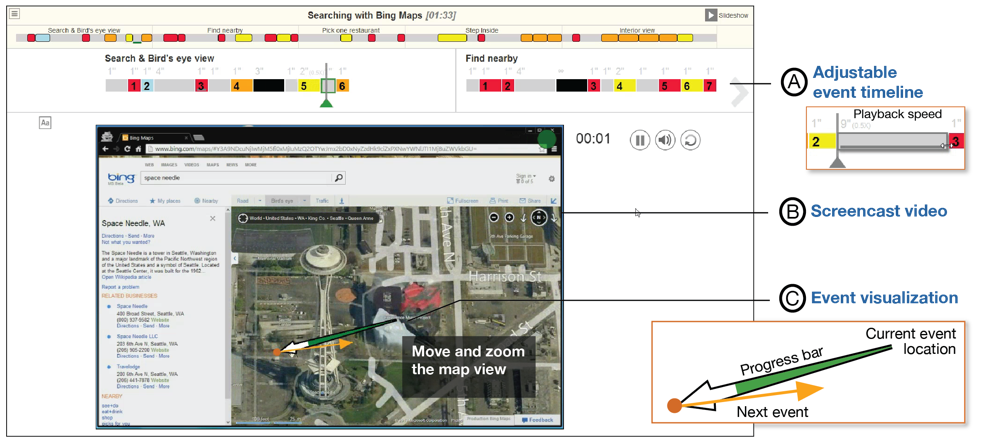
\includegraphics[width=\textwidth]{\demowiz/fig/ui/demowiz_ui}
  \caption{DemoWiz visualizes input events in a screencast video to help presenters anticipate the upcoming event for narrating a software demonstration in a live presentation.}
  \label{fig:demowiz_teaser}
\end{figure*}
